\documentclass[a4paper,12pt,numbers=noenddot]{article}
% 英文字型環境----------------------------------------------------------------
\usepackage{fontspec}%英文字型
% 編號環境----------------------------------------------------------------
% \usepackage{secdot}%section標號後方加上一點
\usepackage{enumitem}%標號巨集
\usepackage{nopageno}
\usepackage[makeroom]{cancel}
\usepackage{listofitems}
\usepackage{amsmath, amsthm, amsfonts, amssymb}
\usepackage{pythonhighlight}
\renewcommand{\Re}{\mathfrak{Re}}
\renewcommand{\Im}{\mathfrak{Im}}
% \usepackage[T1]{fontenc}
% \usepackage{mathptmx}
% \DeclareMathAlphabet{\mathcal}{OMS}{cmsy}{m}{n}
% \DeclareSymbolFont{largesymbols}{OMX}{cmex}{m}{n}
\usepackage{colortbl}
\usepackage{multirow}
\usepackage{arydshln}
\usepackage[colorinlistoftodos]{todonotes}
\usepackage[colorlinks,linkcolor=blue]{hyperref}
\hypersetup{hidelinks,          % 隱藏邊框
            colorlinks=true,    % 啟用彩色連結
            linkcolor=black,    % 目錄、圖片等內部連結為黑色
            citecolor=blue,    % 參考文獻連結為黑色
            filecolor=black,    % 檔案連結為黑色
            urlcolor=blue,      % URL 連結為藍色
            pdfstartview=Fit,
            breaklinks=true
}

\usepackage{graphicx}
\usepackage{pgfplots}
\usepackage{tikzpeople}
\usepackage{tcolorbox}
\tcbuselibrary{skins}
\usepackage{listings}
\usepackage{xcolor}
\usepackage{makecell}
\usepackage{tabularx}
\parindent=0pt
\usepackage{tikz}
\usetikzlibrary{tikzmark}
\usetikzlibrary{matrix}

\usepackage{fancyhdr}
\fancypagestyle{firstpagestyle}{
\cfoot{}
\fancyhead[R]{}
\fancyhead[L]{}
\fancyfoot[C]{\thepage}
\renewcommand{\headwidth}{18cm}
\renewcommand{\headrulewidth}{0pt}
\renewcommand{\footrulewidth}{1pt}}

\fancypagestyle{secondpagestyle}{
\cfoot{}
\fancyhead[R]{}
\fancyhead[L]{}
\fancyfoot[C]{\thepage}
\renewcommand{\headwidth}{18cm}
\renewcommand{\headrulewidth}{1pt}
\renewcommand{\footrulewidth}{1pt}}

\fancypagestyle{evenpagestyle}{
\cfoot{}
\fancyhead[R]{Fall 2025, Introduction to Algebra (I)}
\fancyhead[L]{Preview Note}
\fancyfoot[R]{Atmospheric Sciences, National Taiwan University}
\fancyfoot[L]{Page \thepage\ of\ 20}
\renewcommand{\headwidth}{18cm}
\renewcommand{\headrulewidth}{1pt}
\renewcommand{\footrulewidth}{1pt}}

\fancypagestyle{oddpagestyle}{
\cfoot{}
\fancyhead[L]{Fall 2025, Introduction to Algebra (I)}
\fancyhead[R]{Preview Note}
\fancyfoot[L]{Atmospheric Sciences, National Taiwan University}
\fancyfoot[R]{Page \thepage\ of\ 20}
\renewcommand{\headwidth}{18cm}
\renewcommand{\headrulewidth}{1pt}
\renewcommand{\footrulewidth}{1pt}}

\definecolor{codegreen}{rgb}{0,0.8,0}
\definecolor{codegray}{rgb}{0.8,0.8,0.8}
\definecolor{codepurple}{rgb}{0.58,0,0.82}
\definecolor{codered}{rgb}{1.0,0,0.0}
\definecolor{backcolor}{rgb}{0.85,1.0,1.0}
\definecolor{rain}{rgb}{0.1,0.54,1.0}
\definecolor{sky}{rgb}{0.6,0.75,0.95}

\colorlet{myred}{red!80!black}
\colorlet{myblue}{blue!80!black}
\colorlet{mygreen}{green!60!black}
\colorlet{myorange}{orange!80!black!80}

\lstdefinestyle{mystyle}{
    backgroundcolor=\color{backcolor},   
    commentstyle=\color{codegreen},
    keywordstyle=\color{rain},
    numberstyle=\color{gray}\scriptsize,
    stringstyle=\color{codered},
    basicstyle=\ttfamily\footnotesize,
    breakatwhitespace=false,         
    breaklines=ture,                 
    captionpos=b,                    
    keepspaces=true,                 
    numbers=left,                    
    numbersep=5pt,                  
    showspaces=false,                
    showstringspaces=false,
    showtabs=false,                  
    tabsize=2
}
\lstset{style=mystyle}

\NewTotalTColorBox[auto counter]{\Theorem}{ +m +m +m }{ 
    notitle,
    colback=red!6!white,
    colbacklower=white,
    frame hidden,
    boxrule=0pt,
    bicolor,
    sharp corners,
    borderline west={4pt}{0pt}{red!50!white},
}{
    \textcolor{red!50!white}{
        \sffamily
        \textbf{Theorem #1 }%
    }%
    #2
    \tcblower%
    \textcolor{red!50!white}{
        \sffamily
        \textbf{Proof. }%
    }%
    #3
}

\NewTotalTColorBox[auto counter]{\Definition}{ +m +m }{ 
    notitle,
    colback=blue!10!green!5!white,
    frame hidden,
    boxrule=0pt,
    enhanced,
    sharp corners,
    borderline west={4pt}{0pt}{green!60!blue},
}{
    \textcolor{green!60!blue}{
        \sffamily
        \textbf{Definition #1 }%
    }%
    #2
}

\NewTotalTColorBox[auto counter]{\Proposition}{ +m +m +m }{ 
    notitle,
    colback=brown!10!orange!5!white,
    colbacklower=white,
    frame hidden,
    boxrule=0pt,
    bicolor,
    sharp corners,
    borderline west={4pt}{0pt}{orange!20!brown},
}{
    \textcolor{orange!20!brown}{
        \sffamily
        \textbf{Proposition #1 }%
    }%
    #2
    \tcblower%
    \textcolor{orange!20!brown}{
        \sffamily
        \textbf{Proof. }%
    }%
    #3
}

\NewTotalTColorBox[auto counter]{\Example}{ +m +m +m }{ 
    notitle,
    colback=blue!5!white,
    colbacklower=white,
    frame hidden,
    boxrule=0pt,
    bicolor,
    sharp corners,
    borderline west={4pt}{0pt}{blue!60!black},
}{
    \textcolor{blue!60!black}{
        \sffamily
        \textbf{Example #1 }%
    }%
    #2
    \tcblower%
    \textcolor{blue!60!black}{
        \sffamily
        \textbf{Sol. }%
    }%
    #3
}

\NewTotalTColorBox[auto counter]{\Exam}{ +m +m }{ 
    notitle,
    colback=blue!5!white,
    frame hidden,
    boxrule=0pt,
    enhanced,
    sharp corners,
    borderline west={4pt}{0pt}{blue!60!black},
}{
    \textcolor{blue!60!black}{
        \sffamily
        \textbf{Example #1 }%
    }%
    #2
}

\NewTotalTColorBox[auto counter]{\Proppf}{ +m }{ 
    notitle,
    colback=white,
    colbacklower=white,
    frame hidden,
    boxrule=0pt,
    bicolor,
    sharp corners,
    borderline west={4pt}{0pt}{orange!20!brown},
}{
    \textcolor{orange!20!brown}{
    }%
    #1
}

\usepackage{caption}
\captionsetup{
    justification=centering
}

\newcommand{\abs}[1]{\left\vert #1 \right\vert}
\newcommand{\mb}[1]{\mathbb{#1}}
\newcommand{\mc}[1]{\mathcal{#1}}

% 每段文字的行頭縮排2個字 -----------------------------------
\usepackage{indentfirst}
\linespread{1.2}\selectfont
\setlength{\parindent}{0pt}

% 版面環境----------------------------------------------------------------
\usepackage{geometry}%版面設定的巨集
\geometry{headsep=20pt}
\geometry{%版面設定
a4paper,
total={210mm,297mm}, %寬210mm,長297mm
top=20mm, % 上下左右的空白寬
bottom=20mm,
left=15mm,
right=15mm}

%內容開始 ----------------------------------------------------------------
\begin{document}
\thispagestyle{firstpagestyle}
\pagenumbering{roman}
\begin{center}
{\bf\large Fall 2025\hspace{4pt} Introduction to Algebra (I)}

\vspace{10pt}
{\bf\large Preview Note}

\vspace{10pt}
{Department : Atmospheric Sciences\hspace{10pt}
Name : Guan-Hao, Chen\hspace{10pt}Student ID : B11209022}
\vspace{6pt}
\textcolor{gray}{\rule{\linewidth}{0.5pt}}
\end{center}
\vspace{-25pt}
\thispagestyle{firstpagestyle}
\begin{center}
    \tableofcontents
\end{center}
\newpage
\thispagestyle{oddpagestyle}
\pagenumbering{arabic}
\setcounter{page}{1}
\setcounter{section}{-1}
% ==============================================================================
\section{Preliminaries}
\subsection{Basics}
The subset of a given set $A$ is
\begin{align*}
    B = \{a\in A\ |\ \dots\text{(conditions on a)}\dots\}
\end{align*}
The {\sl order} (or {\sl cardinality}) of a set $A$ will be denoted by $\abs{A}$.
If $A$ is a finite set, the order of $A$ is simply the number of elements of $A$.

The {\sl Cartesian product} of two sets $A$ and $B$ is the collation $A\times B = \{(a,b)\ |\ a\in A,b\in B\}$,
of ordered pairs of elements from $A$ and $B$.

The following notation for some common sets of numbers
\begin{enumerate}[leftmargin=20pt, itemsep=0pt, topsep=3pt]
    \item {\bf Integers}: $\mb{Z} = \{0,\pm 1, \pm 2,\dots\}$.
    \item {\bf Rational numbers}: $\mb{Q} = \{a/b\ |\ a,b\in\mb{Z},b\neq 0\}$.
    \item {\bf Real numbers}: $\mb{R} = \{\text{all decimal expansions} \pm d_{1}d_{2}\dots d_{n}.a_{1}a_{2}a_{3}\dots\}$.
    \item {\bf Complex numbers}: $\mb{C} = \{a+bi\ |\ a,b\in\mb{R},i^{2}=-1\}$.
    \item $\mb{Z}^{+}$, $\mb{Q}^{+}$ and $\mb{R}^{+}$ will denote the positive (nonzero) elements in $\mb{Z}$, $\mb{Q}$ and $\mb{R}$, respectively.
\end{enumerate}
The notation $f:A\to B$ or $A\xrightarrow{\,f\,} B$ to denote a {\sl function} (or {\sl map}) $f$ from $A$ to $B$,
and the value of $f$ at $a$ is denoted by $f(a)$.
The set $A$ is called the {\sl domain} of $f$ and
$B$ is called the {\sl codomain} of $f$.

The notation $f:a\mapsto b$ or $a\mapsto b$ if $f$ is understood indicates that $f(a)=b$, i.e., the function is being specified on {\sl elements}.
If the function $f$ is not specified on elements, it is important in general to check
that $f$ is {\sl well defined}, i.e., is unambiguously determined.

The set
\begin{align*}
    f(A) = \{b\in B\ |\ b=f(a)\text{, for some }a\in A\}
\end{align*}
is a subset of $B$, called the {\sl range} or {\sl image} of $f$ (or the {\sl image} of $A$ under $f$).

For each subset $C$ of $B$, the set
\begin{align*}
    f^{-1}(C) = \{a\in A\ |\ f(a)\in C\}
\end{align*}
consisting of the elements of $A$ mapping into $C$ under $f$ is called
the {\sl preimage} or {\sl inverse image} of $C$ under $f$.
For each $b\in B$, the preimage of $\{b\}$ under $f$ is called the {\sl fiber} of $f$ over $b$.
Note that $f^{-1}$ is not in general a function and that the fibers of $f$ generally
contain many elements since there may be many elements of $A$ mapping to the element $b$.

If $f:A\to B$ and $g:B\to C$, then the composite map $g\circ f:A\to C$ is defined by
\begin{align*}
    (g\circ f)(a) = g(f(a))
\end{align*}
\newpage
\thispagestyle{evenpagestyle}
\Definition{0.1-1}
{Let $f:A\to B$
\begin{enumerate}[leftmargin=20pt, itemsep=0pt, topsep=3pt]
    \item $f$ is {\sl injective} or is an {\sl injection} if whenever $a_{1}\neq a_{2}$, then $f(a_{1})\neq f(a_{2})$.
    \item $f$ is {\sl surjective} or is a {\sl surjection} if for all $b\in B$, there is some $a\in A$ such that $f(a)=b$.
    \item $f$ is {\sl bijective} or is a {\sl bijection} if it is both injective and surjective.
    If such a bijection $f$ exists from $A$ to $B$, we say $A$ and $B$ are in {\sl bijective correspondence}.
    \item $f$ has a {\sl left inverse} if there is a function $g:B\to A$ such that $g\circ f: A\to A$ is the identity map on $A$, i.e., $(g\circ f)(a)=a$ for all $a\in A$.
    \item $f$ has a {\sl right inverse} if there is a function $h:B\to A$ such that $f\circ h: B\to B$ is the identity map on $B$, i.e., $(f\circ h)(b)=b$ for all $b\in B$.
\end{enumerate}}

\Proposition{0.1-1}
{Let $f:A\to B$
\begin{enumerate}[leftmargin=20pt, itemsep=0pt, topsep=3pt]
    \item The map $f$ is injective if and only if $f$ has a left inverse.
    \item The map $f$ is surjective if and only if $f$ has a right inverse.
    \item The map $f$ is a bijection if and only if there exists $g:B\to A$ such 
    that $f \circ g$ is the identity map on $B$ and $g \circ f$ is the identity map on $A$.
    \item If $A$ and $B$ are finite sets with the same number of elements (i.e., $\abs{A} = \abs{B}$),
    then $f : A \to B$ is bijective if and only if $f$ is injective if and only if $f$ is surjective.
\end{enumerate}}
{\begin{enumerate}[leftmargin=20pt, itemsep=0pt, topsep=3pt]
    \item ($\Rightarrow$) Suppose $f$ is injective. Notice that if $b\in f(A)$ then there is a unique $a\in A$ such that
    
    $f(a)=b$. Choose any $a_{0}\in A$, and define $g:B\to A$ by
    \linespread{1}\selectfont
    \begin{align*}
        g(b) = \begin{cases}
            a & \text{if } b\in f(A) \\
            a_{0} & \text{if } b\notin f(A)
        \end{cases}
    \end{align*}
    \linespread{1.2}\selectfont
    Then $(g\circ f)(a) = a$ for all $a\in A$, so $g$ is a left inverse of $f$.
    
    ($\Leftarrow$) Suppose $f$ has a left inverse $g$, and that $f(a) = f(b)$.
    Then $g(f(a)) = g(f(b))$, and since $g\circ f:A\to A$, we have $a=b$, which shows $f$ is injective.
    \item ($\Rightarrow$) Suppose $f$ is surjective. Then every $b\in B$ is in the image of $f$, so for each $b\in B$
    pick an element $g(b)\in A$ such that $f(g(b))=b$. Then $g$ is a right inverse of $f$.

    ($\Leftarrow$) Suppose $f$ has a right inverse $g$ and let $b\in B$. Then $f(g(b))=b$ as $f\circ g: B\to B$.
    This shows $b\in f(A)$, so $f(A) = B$ and $f$ is surjective.
    \item ($\Rightarrow$) Suppose $f$ is a bijection, then $f$ is injective and surjective by definition.
    By part 1. there exists a left inverse $g:B\to A$ such that $g\circ f:A\to A$,
    and by part 2. there exists a right inverse $g:B\to A$ such that $f\circ g:B\to B$.
    
    ($\Leftarrow$) Suppose there exists $g:B\to A$ such that $f\circ g:B\to B$ and $g\circ f:A\to A$.
    Then by part 1., $f$ is surjective, and by part 2., $f$ is injective.
    Then $f$ is a bijection.
\end{enumerate}
}
\newpage
\thispagestyle{oddpagestyle}
\Proppf
{\begin{enumerate}[leftmargin=20pt, itemsep=0pt, topsep=0pt]
    \setcounter{enumi}{3}
    \item {\bf Claim}:
    \begin{itemize}[leftmargin=20pt, itemsep=0pt, topsep=3pt]
        \item [(1)] If $f:A \to B$ is injective, then $\abs{A} \leq \abs{B}$.
        \item [(2)] If $f:A \to B$ is surjective, then $\abs{A} \geq \abs{B}$.
        \item [(3)] If $f:A \to B$ is a bijection, then $\abs{A} = \abs{B}$.
    \end{itemize}
    {\it proof}. Let $A=\{a_{1},a_{2},\dots,a_{m}\}$ has $m$ elements.
    \begin{itemize}[leftmargin=20pt, itemsep=0pt, topsep=3pt]
        \item [(1)] $\{f(a_{1}),f(a_{2}),\dots,f(a_{m})\}$ is a subset of $B$, because $f$ is injective, $\abs{A} = m \leq \abs{B}$.
        \item [(2)] $\{f(a_{1}), f(a_{2}),\dots,f(a_{m})\}=B$ has at most $m$ different elements because $f$ is surjective, $\abs{A} = m \geq \abs{B}$.
        \item [(3)] This follows from (1) and (2), since $\abs{A} \leq \abs{B}$ and $\abs{A} \geq \abs{B}$, we have $\abs{A} = \abs{B}$.
    \end{itemize}
\end{enumerate}
}
The situation of part 3. of \textbf{\textsf{\color{orange!20!brown} Proposition 0.1-1}}, 
the map $g$ is necessarily unique and we shall say $g$ is the {\sl 2-sided inverse} (or {\sl inverse}) of $f$.

A {\sl permutation} of a set $A$ is simply a bijection from $A$ to itself.

If $A\subseteq B$ and $f:B\to C$, we denote the {\sl restriction} of $f$ to $A$ by $f|_{A}$.

If $A\subseteq B$ and $g:A\to C$ and there is a function $f:B\to C$ such that $f|_{A}=g$, we shall say $f$ is an {\sl extension} of $g$ to $B$.
\Definition{0.1-2}
{Let $A$ be a nonempty set.
\begin{enumerate}[leftmargin=20pt, itemsep=0pt, topsep=3pt]
    \item A {\sl binary relation} on a set $A$ is a subset $R$ of $A\times A$ and we write $a\sim b$ if $(a,b)\in R$.
    \item The relation $\sim$ on $A$ is said to be:
    \begin{enumerate}[leftmargin=20pt, itemsep=0pt, topsep=0pt, label=(\alph*)]
        \item {\sl reflexive} if $a\sim a$, for all $a\in A$
        \item {\sl symmetric} if $a\sim b$ implies $b\sim a$ for all $a,b\in A$
        \item {\sl transitive} if $a\sim b$ and $b\sim c$ implies $a\sim c$ for all $a,b,c\in A$
    \end{enumerate}
    A relation is an {\sl equivalence relation} if it is reflexive, symmetric and transitive.
    \item If $\sim$ defines an equivalence relation on $A$, then the {\sl equivalence class} of $a\in A$ is defined
    to be $\{x\in A\ |\ x\sim a\}$. Elements of the equivalence class of $a$ are said to be {\sl equivalent} to $a$.
    If $C$ is an equivalence class, any element of $C$ is called a {\sl representative} of the class $C$.
    \item A {\sl partition} of $A$ is any collection $\{A_{i}\ |\ i\in I\}$ of nonempty subsets of $A$ ($I$ some indexing set)
    such that
    \begin{enumerate}[leftmargin=20pt, itemsep=0pt, topsep=0pt, label=(\alph*)]
        \item $A = \cup_{i\in I}A_{i}$
        \item $A_{i} \cap A_{j} = \varnothing$ for all $i,j\in I$ with $i\neq j$, i.e.,
        $A$ is the disjoint union of the sets in the partition.
    \end{enumerate}
\end{enumerate}
}
\newpage
\thispagestyle{evenpagestyle}
\Proposition{0.1-2}
{Let $A$ be a nonempty set.
\begin{enumerate}[leftmargin=20pt, itemsep=0pt, topsep=3pt]
    \item If $\sim$ defines an equivalence relation on $A$, then the set of equivalence classes of $\sim$ form a partition of $A$.
    \item If $\{A_{i}\ |\ i\in I\}$ is a partition of $A$, then there is an equivalence relation on $A$ whose equivalence classes are precisely the sets $A_{i}$, $i\in I$.
\end{enumerate}}
{
\href{https://math.libretexts.org/Courses/Monroe\_Community\_College/MTH\_220\_Discrete\_Math/6\%3A\_Relations/6.3\%3A\_Equivalence\_Relations\_and\_Partitions}
{Link}
}

\subsection{Properties of the integers}
\subsubsection{Well Ordering of \texorpdfstring{$\mb{Z}$}{Z}}
If $A$ is any nonempty subset of $\mb{Z}^{+}$, there is some element $m\in A$ such that
$m\le a$, for all $a\in A$ ($m$ is call a {\sl minimal element} of $A$).

\subsubsection{Divides}
If $a,b\in \mb{Z}$ with $a\neq 0$, we say $a$ {\sl divides} $b$ if there is an element $c\in\mb{Z}$ such that
$b = ac$. In this case, we write $a\mid b$; if $a$ does not divide $b$, we write $a\nmid b$.

\subsubsection{Greatest Common Divisor (g.c.d.)}
If $a,b\in \mb{Z}\,\diagdown\{0\}$, there is a unique positive integer $d$, called the {\sl greatest common divisor} of $a$ and $b$
(or g.c.d. of $a$ and $b$), satisfying:
\begin{enumerate}[leftmargin=20pt, itemsep=0pt, topsep=3pt, label=(\arabic*)]
    \item $d\mid a$ and $d\mid b$ ($d$ is a common divisor of $a$ and $b$)
    \item If $e\mid a$ and $e\mid b$, then $e\le d$ ($d$ is the greatest such divisor)
\end{enumerate}
The g.c.d. of $a$ and $b$ will be denoted by $(a,b)$ (or $\gcd(a,b)$).
If $(a,b)=1$, we say that $a$ and $b$ are {\sl relatively prime}.

\subsubsection{Least Common Multiple (l.c.m.)}
If $a,b\in \mb{Z}\,\diagdown\{0\}$, there is a unique positive integer $l$, called the {\sl least common multiple} of $a$ and $b$
(or l.c.m. of $a$ and $b$), satisfying:
\begin{enumerate}[leftmargin=20pt, itemsep=0pt, topsep=3pt, label=(\arabic*)]
    \item $a\mid l$ and $b\mid l$ ($l$ is a common multiple of $a$ and $b$)
    \item If $a\mid m$ and $b\mid m$, then $l\le m$ ($l$ is the least such multiple)
\end{enumerate}
The l.c.m. of $a$ and $b$ will be denoted by $[a,b]$ (or $\mathrm{lcm}(a,b)$).
The connection between the g.c.d. $d$ and the l.c.m. $l$ of two integers $a$ and $b$ is given by $dl=ab$.

\subsubsection{The Division Algorithm}
If $a,b\in \mb{Z}\,\diagdown\{0\}$, then there exist unique $q,r\in \mb{Z}$ such that
\begin{align*}
    a = qb + r \text{\qquad and \qquad} 0\le r < \abs{b}
\end{align*}
where $q$ is the {\sl quotient} and $r$ is the {\sl remainder}.
\newpage
\thispagestyle{oddpagestyle}

\subsubsection{The Euclidean Algorithm}
If $a,b\in \mb{Z}\,\diagdown\{0\}$, then we obtain a sequence of quotients and remainders
\begin{align*}
    a &= q_{0} b + r_{0}\tag{0}\\
    b &= q_{1} r_{0} + r_{1}\tag{1}\\
    r_{0} &= q_{2} r_{1} + r_{2}\tag{2}\\
    r_{1} &= q_{3} r_{2} + r_{3}\tag{3}\\
    &\vdots\\
    r_{n-2} &= q_{n} r_{n-1} + r_{n}\tag{n}\\
    r_{n-1} &= q_{n+1} r_{n}\tag{$n+1$}
\end{align*}
where $r_{n}$ is the last nonzero reminder. Such an $r_{n}$ exists since
$\abs{b}>\abs{r_{0}}>\abs{r_{1}}>\cdots>\abs{r_{n}}$ is a decreasing sequence of strictly positive integers
if the reminders are nonzero and such a sequence cannot continue indefinitely.
Then $r_{n}$ is the g.c.d. $(a,b)$ of $a$ and $b$.
\Example{0.2.6-1}
{Find the g.c.d. of $a=57970$ and $b=10353$.}
{Applying the Euclidean algorithm, we have
\begin{align*}
    57970 &= (5) 10353 + 6205\\
    10353 &= (1) 6205 + 4148\\
    6205 &= (1) 4148 + 2057\\
    4148 &= (2) 2057 + 34\\
    2057 &= (60) 34 + 17\\
    34 &= (2) 17
\end{align*}
Thus, the g.c.d. of $57970$ and $10353$ is $(57970, 10353) = 17$.
}

\subsubsection{\texorpdfstring{$\mb{Z}\,$}{Z}-linear Combinations}
One consequence of the Euclidean Algorithm which we shall use regularly
is the following: if $a,b\in \mb{Z}\,\diagdown\{0\}$, then there exist $x,y\in\mb{Z}$ such that
\begin{align*}
    (a,b) = ax + by
\end{align*}
that is, {\sl the g.c.d. of $a$ and $b$ is a $\mb{Z}\,$-linear combination of $a$ and $b$}.
This follows by recursively writting the element $r_{n}$ in the Euclidean Algorithm in terms of the previous
remainders (namely, use equation (n) above to solve for $r_{n} = r_{n-2} - q_{n}r_{n-1}$
in terms of the remainders $r_{n-1}$ and $r_{n-2}$, then use equation ($n-1$) to write $r_{n}$
in terms of the remainders $r_{n-2}$ and $r_{n-3}$, etc., eventually writing $r_{n}$ in terms of $a$ and $b$).
\newpage
\thispagestyle{evenpagestyle}
\Example{0.2.7-1}
{Use the Euclidean Algorithm to find integers $x,y$ such that
\begin{align*}
    (57970, 10353) = 57970x + 10353y
\end{align*}
}
{Based on \textbf{\textsf{\color{blue!60!black} Example 0.2.6-1}}
we know that $(57970, 10353) = 17$. Start from the fifth equation in the Euclidean Algorithm,
\begin{align*}
    17 &= 2057 - 60\cdot 34\\
    &= 2057 - 60\cdot (4148 - (2) 2057) = 121\cdot 2057 - 60\cdot 4148\\
    &= 121\cdot (6205 - (1) 4148) - 60\cdot 4148 = 121\cdot 6205 - 181\cdot 4148\\
    &= 121\cdot 6205 - 181\cdot (10353 - (1) 6205) = 302\cdot 6205 - 181\cdot 10353\\
    &= 302\cdot (57970 - (5) 10353) - 181\cdot 10353\\
    &= 302\cdot 57970 + (-1691)\cdot 10353
\end{align*}
Thus, $x=302$ and $y=-1691$ is a solution of $(57970, 10353) = 57970x + 10353y$.
}

\subsubsection{Prime and Composite Numbers}
An element $p$ of $\mb{Z}^{+}$ is called a {\sl prime} if $p>1$ and the only positive divisors of $p$ are $1$ and $p$.
An integer $n>1$ which is not prime is called {\sl composite}.

\subsubsection{The Fundamental Theorem of Arithmetic}
If $n\in\mb{Z}$, $n>1$, then $n$ can be factored uniquely into the product of primes, i.e., there are distinct primes
$p_{1}, p_{2}, \dots, p_{s}$ and positive integers $\alpha_{1}, \alpha_{2},\dots,\alpha_{s}$ such that
\begin{align*}
    n = p_{1}^{\alpha_{1}}p_{2}^{\alpha_{2}}\dots p_{s}^{\alpha_{s}}
\end{align*}
This factorization is unique in the sense that if $q_{1},q_{2},\dots,q_{t}$ are any distinct
primes and positive integers $\beta_{1},\beta_{2},\dots,\beta_{t}$ such that
\begin{align*}
    n = q_{1}^{\beta_{1}}q_{2}^{\beta_{2}}\dots q_{t}^{\beta_{t}}
\end{align*}
then $s=t$ and if we arrange the two sets of primes in increasing order, then $q_{i} = p_{i}$
and $\alpha_{i} = \beta_{i}$ $1\le i\le s$.

Suppose the positive integers $a$ and $b$ are expressed as products of prime powers:
\begin{align*}
    a = p_{1}^{\alpha_{1}}p_{2}^{\alpha_{2}}\dots p_{s}^{\alpha_{s}} \qquad b = p_{1}^{\beta_{1}}p_{2}^{\beta_{2}}\dots p_{s}^{\beta_{s}}
\end{align*}
where $p_{1}, p_{2}, \dots, p_{s}$ are distinct and the exponents are $\ge 0$
(we allow the exponents to be $0$ here, so that the products are taken over the same set of primes -- the exponent will be $0$ if that prime is not actually a divisor).
Then the g.c.d. of $a$ and $b$ is
\begin{align*}
    (a,b) = p_{1}^{\min\{\alpha_{1}, \beta_{1}\}}p_{2}^{\min\{\alpha_{2}, \beta_{2}\}}\dots p_{s}^{\min\{\alpha_{s}, \beta_{s}\}}
\end{align*}
and the l.c.m. of $a$ and $b$ is
\begin{align*}
    [a,b] = p_{1}^{\max\{\alpha_{1}, \beta_{1}\}}p_{2}^{\max\{\alpha_{2}, \beta_{2}\}}\dots p_{s}^{\max\{\alpha_{s}, \beta_{s}\}}
\end{align*}
\newpage
\thispagestyle{oddpagestyle}

\subsubsection{Euler \texorpdfstring{$\varphi\,$}{phi}-function}
For $n\in \mb{Z}^{+}$, let $\varphi(n)$ be the number of positive integers $a\le n$
with $a$ relatively prime to $n$, i.e., $(a,n) = 1$. For example, $\varphi(12) = 4$
since the positive integers $1, 5, 7, 11$ are the only positive integers less than or equal to $12$
which have no factors in common with $12$. For prime $p$, $\varphi(p) = p-1$, and more generally,
for all $a\ge 1$ we have the formula
\begin{align*}
    \varphi(p^{a}) = p^{a} - p^{a-1} = p^{a-1}(p-1)
\end{align*}
The function $\varphi$ is {\sl multiplicative} in the sense that
\begin{align*}
    \varphi(ab) = \varphi(a)\varphi(b)\qquad \text{if } (a,b) = 1
\end{align*}
(note that it is important here that $a$ and $b$ be relatively prime).
Together with the formula above this gives a general formula for the values of $\varphi$ : 
if $n=p_{1}^{\alpha_{1}}p_{2}^{\alpha_{2}}\dots p_{s}^{\alpha_{s}}$, then
\begin{align*}
    \varphi(n) &= \varphi(p_{1}^{\alpha_{1}})\varphi(p_{2}^{\alpha_{2}})\dots\varphi(p_{s}^{\alpha_{s}})\\
    &= p_{1}^{\alpha_{1}-1}(p_{1} - 1) p_{2}^{\alpha_{2}-1}(p_{2} - 1)\dots p_{s}^{\alpha_{s}-1}(p_{s} - 1)
\end{align*}
\Example{0.2.10-1}
{Find the value of $\varphi(36)$.
}
{
The prime factorization of $36$ is $36 = 2^{2}\cdot 3^{2}$, therefore
\begin{align*}
    \varphi(36) &= \varphi(2^{2})\varphi(3^{2})\\
    &= 2^{2-1}(2-1)3^{2-1}(3-1)\\
    &= 2\cdot 1\cdot 3\cdot 2 = 12
\end{align*}
}

\subsection{\texorpdfstring{$\mb{Z}/n\mb{Z}$}{Z/nZ} : The integers modulo \texorpdfstring{$n$}{n}}
Let $n$ be a fixed positive integer. Define a relation on $\mb{Z}$ by
\begin{align*}
    a\sim b\quad\text{if and only if}\quad n\mid (a-b)
\end{align*}
Clearly $a\sim a$, and $a\sim b$ implies $b\sim a$ for any integers $a$ and $b$, so this relation
is trivially reflexive and symmetric. If $a\sim b$ and $b\sim c$, then $n$ divides $a-b$ and $n$ divides $b-c$,
so $n$ also divides the sum of these two integers, i.e., $n$ divides $(a-b)+(b-c) = a-c$, 
so $a\sim c$ and the relation is transitive.
Hence, this is an equivalence relation. Write $a\equiv b\pmod{n}$ (read: $a$ is {\sl congruent} to $b\bmod{n}$) if $a\sim b$.
For any $k\in\mb{Z}$ we shall denote the equivalence class of $a$ by $\overline{a}$ -- this is called the {\sl congruent class}
or {\sl residue class} of $a\bmod{n}$ and consists of the integers which differ from $a$ by an integral multiple of $n$, i.e.,
\begin{align*}
    \overline{a} &= \{a+kn\ |\ k\in\mb{Z}\}\\
    &= \{a, a\pm n, a\pm 2n, a\pm 3n, \dots\}
\end{align*}
There are precisely $n$ distinct equivalence classes mod $n$, namely
\begin{align*}
    \overline{0}, \overline{1}, \overline{2}, \dots, \overline{n-1}
\end{align*}
\newpage
\thispagestyle{evenpagestyle}
determined by the possible remainders after division by $n$, and this residue classes
partition the integers $\mb{Z}$. the set of equivalence classes under this equivalence relation
will be denoted by $\mb{Z}/n\mb{Z}$, and called the {\sl integers modulo $n$} (or the {\sl integers mod $n$}).

The process of finding the equivalence class mod $n$ of some integer $a$ is often
referred to as {\sl reducing $a$ mod $n$}. This terminology also frequently refers to finding the smallest
nonnegative integer congruent to $a\bmod{n}$ (the {\sl least residue} of $a\bmod n$).

\Definition{0.3-1}
{We can define an addition and a multiplication for the elements of $\mb{Z}/n\mb{Z}$,
defining {\sl modular arithmetic} as follows: for $\overline{a},\overline{b}\in\mb{Z}/n\mb{Z}$,
define their sum and product by
\begin{align*}
    \overline{a} + \overline{b} = \overline{a+b}\qquad\text{and}\qquad
    \overline{a} \cdot \overline{b} = \overline{ab}
\end{align*}}
Given any two elements $\overline{a}$ and $\overline{b}$ in $\mb{Z}/n\mb{Z}$, to compute
their sum (respectively, their product) take {\sl any representative} integer $a$ in the
{\sl class} $\overline{a}$ and {\sl any representative} integer $b$ in the {\sl class} $\overline{b}$,
and add (respectively, multiply) the integers $a$ and $b$ as usual in $\mb{Z}$, and then take
the equivalence class containing the result.
\Theorem{0.3-1}
{The operations of addition and multiplication on $\mb{Z}/n\mb{Z}$ defined in \textbf{\textsf{\color{green!60!blue} Definition 0.3-1}}
are both well defined, that is, they do not depend on the choices of representatives for the classes involved.
More precisely, if $a_{1}, a_{2}\in \mb{Z}$ and $b_{1}, b_{2}\in \mb{Z}$ with $\overline{a_{1}} = \overline{b_{1}}$
and $\overline{a_{2}} = \overline{b_{2}}$, then $\overline{a_{1}+a_{2}} = \overline{b_{1} + b_{2}}$ and $\overline{a_{1}a_{2}} = \overline{b_{1}b_{2}}$, i.e., if
\begin{align*}
    a_{1} \equiv b_{1}\pmod{n}
    \qquad\text{and}\qquad
    a_{2} \equiv b_{2}\pmod{n}
\end{align*}
then
\begin{align*}
    a_{1} + a_{2} \equiv b_{1} + b_{2}\pmod{n}
    \qquad\text{and}\qquad
    a_{1}a_{2} \equiv b_{1}b_{2}\pmod{n}
\end{align*}
}
{Suppose $a_{1}\equiv b_{1}\pmod{n}$, i.e., $a_{1}-b_{1}$ is divisible by $n$.
Then $a_{1} = b_{1} + sn$ for some integer $s$.
Similarly, $a_{2}\equiv b_{2}\pmod{n}$ means $a_{2} = b_{2} + tn$ for some integer $t$.
Then $a_{1} + a_{2} = (b_{1} + b_{2}) + (s+t)n$, so $a_{1} + a_{2} \equiv b_{1} + b_{2}\pmod{n}$,
which shows that the sum of the residue classes is independent of the representatives chosen.

Similarly, $a_{1}a_{2} = (b_{1} + sn)(b_{2} + tn) = b_{1}b_{2} + (b_{1}t + b_{2}s + stn)n$,
so $a_{1}a_{2} \equiv b_{1}b_{2}\pmod{n}$, and so the product of the residue classes is also independent of the representatives chosen.
}
\Example{0.3-1}
{Find the last two digits in the number $2^{1000}$.
}
{First observe that the last two digits give the remainder of $2^{1000}$ after we divided by $100$,
so we are interested in the residue class mod $100$ containing $2^{1000}$.
We compute $2^{10} = 1024 \equiv 24\pmod{100}$, so then $2^{20} = (2^{10})^{2}\equiv 24^{2} = 576\equiv 76\pmod{100}$.
Then $2^{40} = (2^{20})^{2}\equiv 76^{2} = 5776\equiv 76\pmod{100}$.
Similarly, $2^{80} \equiv 2^{160} \equiv 2^{320} \equiv 2^{640} \equiv 76\pmod{100}$.
Finally, $2^{1000} = 2^{640}\cdot 2^{320}\cdot 2^{40} \equiv 76\cdot 76\cdot 76 \equiv 76 \pmod{100}$.
Thus, the last two digits of $2^{1000}$ are $76$.
}
\newpage
\thispagestyle{oddpagestyle}
An important subset of $\mb{Z}/n\mb{Z}$ consists of the collection of residue classes which have a multiplicative inverse in $\mb{Z}/n\mb{Z}$:
\begin{align*}
    (\mb{Z}/n\mb{Z})^{\times} = \{\overline{a}\in\mb{Z}/n\mb{Z}\ |\ \text{there exists } \overline{c}\in\mb{Z}/n\mb{Z} \text{ with } \overline{a}\cdot\overline{c} = \overline{1}\}
\end{align*}
\Proposition{0.3-1}
{\begin{align*}
    (\mb{Z}/n\mb{Z})^{\times} = \{\overline{a}\in\mb{Z}/n\mb{Z}\ |\ (a,n) = 1\}
\end{align*}}
{It is easy to see that if any representative of $\overline{a}$ is relatively prime to $n$,
then all representatives are relatively prime to $n$, so that the set on the right in the proposition is well defined.
}
If $a$ is an integer relatively prime to $n$, then the Euclidean Algorithm produces integers $x$ and $y$ satisfying
$ax+ny=1$, hence $ax\equiv 1\pmod{n}$, so that $\overline{x}$ is the multiplicative inverse of $\overline{a}$ in $\mb{Z}/n\mb{Z}$.
This gives an efficient method for computing multiplicative inverses in $\mb{Z}/n\mb{Z}$.
\Example{0.3-2}
{Find the multiplicative inverse of $\overline{17}$ in $\mb{Z}/60\mb{Z}$.
}
{Suppose $n=60$ and $a=17$. Applying the Euclidean Algorithm, we obtain
\begin{align*}
    60 &= (3) 17 + 9\\
    17 &= (1) 9 + 8\\
    9 &= (1) 8 + 1\\
    8 &= (8) 1
\end{align*}
so that $a$ and $n$ are relatively prime, and $(-7)17 + 2\cdot 60 = 1$.
Hence, $\overline{-7}=\overline{53}$ is the multiplicative inverse of $\overline{17}$ in $\mb{Z}/60\mb{Z}$.
}
\newpage
\thispagestyle{evenpagestyle}
\part{Group Theory}
\section{Introduction to Groups}
\subsection{Basic Axioms and Examples}
\Definition{1.1-1}
{\begin{enumerate}[leftmargin=20pt, itemsep=0pt, topsep=3pt]
    \item A {\sl binary operation} $\star$ on a set $G$ is a function $\star:G\times G\to G$.
    For any $a,b\in G$, we shall write $a\star b$ for $\star(a,b)$.
    \item A binary operation $\star$ on a set $G$ is {\sl associative} if for all $a,b,c\in G$,
    we have $a\star (b\star c) = (a\star b)\star c$.
    \item If $\star$ is a binary operation on a set $G$, we say elements $a$ and $b$ of $G$
    {\sl commute} if $a\star b = b\star a$.
    We say $\star$ (or $G$) is {\sl commutative} if for all $a,b\in G$, we have $a\star b = b\star a$.
\end{enumerate}}
\Exam{1.1-1}
{\begin{enumerate}[leftmargin=20pt, itemsep=0pt, topsep=3pt]
    \item $+$ (usual addition) is a commutative binary operation on $\mb{Z}$ (or on $\mb{Q}$, $\mb{R}$, $\mb{C}$ respectively).
    \item $\times$ (usual multiplication) is a commutative binary operation on $\mb{Z}$ (or on $\mb{Q}$, $\mb{R}$, $\mb{C}$ respectively).
    \item $-$ (usual subtraction) is noncommutative binary operation on $\mb{Z}$, where $-(a,b) = a-b$.
    It is not a binary operation on $\mb{Z}^{+}$ (nor $\mb{Q}^{+}$, $\mb{R}^{+}$) (e.g. $-(1,2) = 1-2 = -1 \notin \mb{Z}^{+}$).
    \item Taking the vector cross-product of two vectors in $\mb{R}^{3}$ is a binary operation which is not associative and not commutative. For example,
    \begin{enumerate}[leftmargin=20pt, itemsep=0pt, topsep=0pt, label=(\arabic*)]
        \item ${\bf u} = (1,2,3)$, ${\bf v} = (4,5,6)\in\mb{R}^{3}$, ${\bf u}\times{\bf v} = (-3, 6, -3)$
        
        $\Rightarrow \mb{R}^{3}\times\mb{R}^{3}\to \mb{R}^{3}$
        \item ${\bf u} = (1,2,3)$, ${\bf v} = (4,5,6)\in\mb{R}^{3}$, ${\bf u}\times{\bf v} = (-3, 6, -3)$, ${\bf v}\times{\bf u} = (3, -6, 3)$
        
        $\Rightarrow$ it is not commutative.
        \item ${\bf u} = (1,2,3)$, ${\bf v} = (4,5,6)$, ${\bf w} = (7,8,9)\in\mb{R}^{3}$,
        
        $({\bf u}\times{\bf v})\times{\bf w} = (-3, 6, -3)\times(7,8,9) = (78,6,-66)$

        ${\bf u}\times({\bf v}\times{\bf w}) = (1,2,3)\times(-3,6,-3) = (-24,-6,12)$
    \end{enumerate}
\end{enumerate}
}
Suppose that $\star$ is a binary operation on a set $G$, and $H$ is a subset of $G$.
If the restriction of $\star$ to $H$ is a binary operation on $H$ ($\forall\ a,b\in H, a\star b\in H$), we say that $H$ is {\sl closed} under $\star$.

Observe that if $\star$ is an associative (respectively, commutative) binary operation on a set $G$,
and $\star$ restricted to some subset $H$ of $G$ is a binary operation on $H$,
then $\star$ is automatically associative (respectively, commutative) on $H$ as well.
\newpage
\thispagestyle{oddpagestyle}
\Definition{1.1-2}
{
\begin{enumerate}[leftmargin=20pt, itemsep=0pt, topsep=3pt]
    \item A {\sl group} is an ordered pair $(G,\star)$ where $G$ is a set and
    $\star$ is a binary operation on $G$ satisfying the following axioms:
    \begin{enumerate}[leftmargin=20pt, itemsep=0pt, topsep=0pt, label=(\roman*)]
        \item {\bf Associative}: $(a\star b)\star c = a\star (b\star c)$, for all $a,b,c\in G$.
        \item {\bf Identity}: There exists an element $e\in G$ such that
        $e\star a = a\star e = a$ for all $a\in G$.
        \item {\bf Inverses}: For each $a\in G$, there exists $a^{-1}\in G$ such that
        $a\star a^{-1} = a^{-1}\star a = e$.
    \end{enumerate}
    \item The group $(G,\star)$ is called {\sl abelian} (or {\sl commutative}) if $a\star b = b\star a$ for all $a,b\in G$.
\end{enumerate}
}
We say $G$ is a {\sl finite group} if in addition $G$ is a finite set.

Note that the axiom (ii) ensures that a group is always nonempty.
\Exam{1.1-2}
{
\begin{enumerate}[leftmargin=20pt, itemsep=0pt, topsep=3pt]
    \item $\mb{Z}, \mb{Q}, \mb{R}$ and $\mb{C}$ are groups under $+$ with $e=0$ and $a^{-1} = -a$ for all $a$.
    \item $\mb{Q}\,\diagdown\{0\}, \mb{R}\,\diagdown\{0\},\mb{C}\,\diagdown\{0\}, \mb{Q}^{+}, \mb{R}^{+}$ are groups
    under $\times$ with $e=1$ and $a^{-1} = \dfrac{1}{a}$.
    \item The axioms for a vector space $V$ which specify that $(V,+)$
    is an abelian group.
    \item For $n\in \mb{Z}^{+}$, $\mb{Z}/n\mb{Z}$ is an abelian group under the operation $+$ with the identity element $\overline{0}$
    and the inverse of $\overline{a}$ is $\overline{-a}$.
    \item For $n\in \mb{Z}^{+}$, the set $(\mb{Z}/n\mb{Z})^{\times}$ of equivalence classes $\overline{a}$ which have multiplicative inverses
    mod $n$ is an abelian group under multiplication with the identity element $\overline{1}$.
\end{enumerate}
}
If $(A,\star)$ and $(B,\diamond)$ are groups, we can find a new group $A\times B$, called the {\sl direct product}, whose elements are those in the Cartesian product
\begin{align*}
    A\times B = \{(a,b)\ |\ a\in A, b\in B\}
\end{align*}
and whose operation is defined componentwise:
\begin{align*}
    (a_{1}, b_{1})(a_{2}, b_{2}) = (a_{1}\star a_{2}, b_{1}\diamond b_{2})
\end{align*}
\Proposition{1.1-1}
{If $G$ is a group under the operation $\star$, then
\begin{enumerate}[leftmargin=20pt, itemsep=0pt, topsep=3pt]
    \item The identity of $G$ is unique.
    \item For each $a\in G$, $a^{-1}$ is uniquely determined.
    \item $(a^{-1})^{-1} = a$ for all $a\in G$.
    \item $(a\star b)^{-1} = (b)^{-1}\star(a)^{-1}$
    \item {\bf Generalized Associative Law}: For any $a_{1}, a_{2},\dots,a_{n}\in G$, the value of $a_{1}\star a_{2}\star\dots\star a_{n}$
    is independent of how the expression is bracketed.
\end{enumerate}
}
{\begin{enumerate}[leftmargin=20pt, itemsep=0pt, topsep=3pt]
    \item If $f$ and $g$ are both identities, then by axiom (ii) of the \textbf{\textsf{\color{green!60!blue} Definition 1.1-2}},
    we have $f\star g = f$ and $g\star f = g$. Thus $f=g$, and the identity is unique.
\end{enumerate}}
\newpage
\thispagestyle{evenpagestyle}
\Proppf
{\begin{enumerate}[leftmargin=20pt, itemsep=0pt, topsep=0pt]
    \setcounter{enumi}{1}
    \item Assume $b$ and $c$ are both inverses of $a$, and let $e$ be the identity of $G$.
    By axiom (iii) of the \textbf{\textsf{\color{green!60!blue} Definition 1.1-2}}, $a\star b=e$ and $c\star a=e$.
    Thus
    \begin{align*}
        c &= c\star e \hspace{10pt}&(\text{Axiom (ii)})\\
        &= c\star (a\star b) \hspace{10pt}&(\text{Since } e = a\star b)\\
        &= (c\star a)\star b \hspace{10pt}&(\text{Axiom (i)})\\
        &= e\star b \hspace{10pt}&(\text{Since } e = c\star a)\\
        &= b \hspace{10pt}&(\text{Axiom (ii)})
    \end{align*}
    \item The inverse of $a$ is $a^{-1}$, and the inverse of $a^{-1}$ is $(a^{-1})^{-1}$, by part 2.,
    we know $a = (a^{-1})^{-1}$.
    \item Let $c = (a\star b)^{-1}$, so by definition of $c$, $(a\star b) \star c = e$.
    By the associative law, we have
    \begin{align*}
        a\star (b\star c) &= e
    \end{align*}
    Multiply both sides on the left by $a^{-1}$ to get
    \begin{align*}
        a^{-1}\star(a\star (b\star c)) = a^{-1}\star e
    \end{align*}
    The associative law on the LHS and the definition of $e$ on the RHS give
    \begin{align*}
        (a^{-1}\star a)\star (b\star c) &= a^{-1}\\
        e\star (b\star c) &= a^{-1}\\
        b\star c &= a^{-1}
    \end{align*}
    Now, multiply both sides on the left by $b^{-1}$ to get
    \begin{align*}
        b^{-1}\star(b\star c) &= b^{-1}\star a^{-1}\\
        (b^{-1}\star b)\star c &= b^{-1}\star a^{-1}\\
        e\star c &= b^{-1}\star a^{-1}\\
        c &= b^{-1}\star a^{-1}
    \end{align*}
    Thus $(a\star b)^{-1} = b^{-1}\star a^{-1}$.
    \item First show the result is true for $n=1,2$ and $3$.
    Next, assume for any $k<n$ that any braketing of a product of $k$ elements,
    $b_{1}\star b_{2}\star \dots\star b_{k}$ can be reduced (without altering the value of the product)
    to an expression of the form
    \begin{align*}
        b_{1}\star(b_{2}\star (b_{3}\star (\dots \star b_{k}))\dots)
    \end{align*}
    Now argue that an bracketing of the product $a_{1}\star a_{2}\star\dots\star a_{n}$ must break into $2$
    subproducts, say $(a_{1}\star a_{2}\star\dots\star a_{k})\star (a_{k+1}\star a_{k+2}\star\dots\star a_{n})$,
    where each subproduct is bracketed in some fashion.
    Apply the induction assumption to each of these two subproducts and finally reduce the result to the form
    $a_{1}\star(a_{2}\star (a_{3}\star (\dots\star a_{n}))\dots)$ to complete the induction.
\end{enumerate}}
\newpage
\thispagestyle{oddpagestyle}
For any group $G$ (operation $\cdot$ implied)
and $x\in G$ and $n\in\mb{Z}^{+}$ since the product $xx\dots x$ ($n$ terms)
does not depend on how it is bracketed, we shall denote it by $x^{n}$.
Denote $x^{-1}x^{-1}\dots x^{-1}$ ($n$ terms) by $x^{-n}$. Let $x^{0} = 1$, the identity of $G$.

When we are dealing with specific groups, we shall use the natural (given) operation.
For example, when the operation is $+$, the identity will be denoted by $0$
and for any element $a$, the inverse $a^{-1}$ will be written $-a$,
and $a+a+\dots+a$ ($n>0$ terms) will be written $na$; $-a-a-\dots-a$ ($n$ terms)
will be written $-na$, and $0a = 0$.
\Proposition{1.1-2}
{Let $G$ be a group and let $a,b\in G$. The equations $ax=b$ and $ya=b$
have unique solutions for $x,y\in G$.
In particular, the left and right cancellation laws hold in $G$, i.e.,
\begin{enumerate}[leftmargin=20pt, itemsep=0pt, topsep=0pt]
    \item If $au=av$, then $u=v$.
    \item If $ub=vb$, then $u=v$.
\end{enumerate}}
{We can solve $ax=b$ by multiplying both sides on the left by $a^{-1}$ and simplifying to get $x=a^{-1}b$.
The uniqueness of $x$ follows because $a^{-1}$ is unique.
Similarly, we can solve $ya=b$ by multiplying both sides on the right by $b^{-1}$ and simplifying to get $y=ba^{-1}$.
The uniqueness of $y$ follows because $b^{-1}$ is unique.

If $au=av$, multiply both sides on the left by $a^{-1}$, and simplify to get $u=v$.
Similarly, if $ub=vb$, multiply both sides on the right by $b^{-1}$, and simplify to get $u=v$.
}

\Definition{1.1-3}
{For $G$ a group and $x\in G$ define the {\sl order} of $x$ to be the smallest positive
integer $n$ such that $x^{n} = 1$, and denote this integer by $\abs{x}$. In this case $x$
is said to be of order $n$. If no positive power of $x$ is the identity, the order of $x$ is defined to be infinity
and $x$ is said to be of infinite order.}

\Exam{1.1-3}
{\begin{enumerate}[leftmargin=20pt, itemsep=0pt, topsep=0pt]
    \item An element of a group has order $1$ if and only if it is the identity.
    \item In the additive groups $\mb{Z}$, $\mb{Q}$, $\mb{R}$ or $\mb{C}$ every nonzero
    element has infinite order.
    \item In the multiplicative groups $\mb{R}\ \diagdown\{0\}$ or $\mb{Q}\ \diagdown\{0\}$ the element
    $-1$ has order $2$ and all other nonidentity elements have infinite order.
    \item In the additive group $\mb{Z}/9\mb{Z}$, the element $\overline{6}$ has order $3$
    since $\overline{6}\neq \overline{0}$, $\overline{6} + \overline{6} = \overline{12} = \overline{3} \neq \overline{0}$,
    but $\overline{6} + \overline{6} + \overline{6} = \overline{18} = \overline{0}$, the identity in this group.
    \item In the multiplicative group $(\mb{Z}/7\mb{Z})^{\times}$, the element $\overline{2}$ has order $3$
    since $\overline{2}\neq \overline{1}$, $\overline{2}\times \overline{2} = \overline{4}\neq \overline{1}$,
    but $\overline{2}\times \overline{2}\times \overline{2} = \overline{8} = \overline{1}$, the identity in this group.
\end{enumerate}
}

\Definition{1.1-4}
{Let $G=\{g_{1},g_{2},\dots,g_{n}\}$ be a finite group with $g_{1} = 1$.
The {\sl multiplication table} or {\sl group table} of $G$ is the $n\times n$ matrix
whose $i$, $j$ entry is the group element $g_{i}g_{j}$.
}
More about the group table:
\begin{enumerate}[leftmargin=20pt, itemsep=0pt, topsep=0pt]
    \item \href{https://youtu.be/BwHspSCXFNM?si=1ucTvpLN6bGUYX9v}{Group Multiplication Tables | Cayley Tables (Abstract Algebra)}
    \item \href{https://youtu.be/tGCqP2ytP14?si=3P4tafGvrpjJWQyd}{Group Theory Step-by-Step: 1 - 7}
\end{enumerate}

\newpage
\thispagestyle{evenpagestyle}
\subsection{Dihedral Groups}
For each $n\in \mb{Z}^{+}$, $n\ge 3$ let $D_{2n}$ be the set of symmetries
of a regular $n$-gon, where a symmetry is any rigid motion of the $n$-gon which can
be effected by taking a copy of the $n$-gon, moving this copy in any fashion in $3$-space,
then placing the copy back on the original $n$-gon so it exactly covers it.

Each symmetry $s$ can be described uniquely by the corresponding permutation $\sigma$
of $\{1,2,3,\dots,n\}$ where if the symmetry $s$ puts vertex $i$ in the place where vertex $j$
was originally, then $\sigma$ is the permutation sending $i$ to $j$.

The identity og $D_{2n}$ is the identity symmetry (which leaves all vertices fixed), denoted by $1$,
and the inverse of $s\in D_{2n}$ is the symmetry which reverses all rigid motions of $s$
(so if $s$ effects permutation $\sigma$, then the inverse of $s$ effects the permutation $\sigma^{-1}$).

\Proposition{1.2-1}
{The order of the dihedral group
\begin{align*}
    \abs{D_{2n}} = 2n
\end{align*}
}
{To find the order $\abs{D_{2n}}$ observe that given any vertex $i$,
there is a symmetry which sends vertex $1$ into position $i$.
Since vertex $2$ is adjacent to vertex $1$, vertex $2$ must end up in position $i+1$ or $i-1$
(when $n+1$ is $1$ and $1-1$ is $n$, i.e., the integers labelling the vertices are read mod $n$).
Moreover, by following the first symmetry by a reflection about the line through vertex $i$ and the center
of the $n$-gon one sees that vertex $2$ can be sent to either position $i+1$ or $i-1$ by some symmetry.
Thus there are $2n$ positions the ordered pair of $1,2$ may be sent to upon applying symmetries.}
\begin{center}
    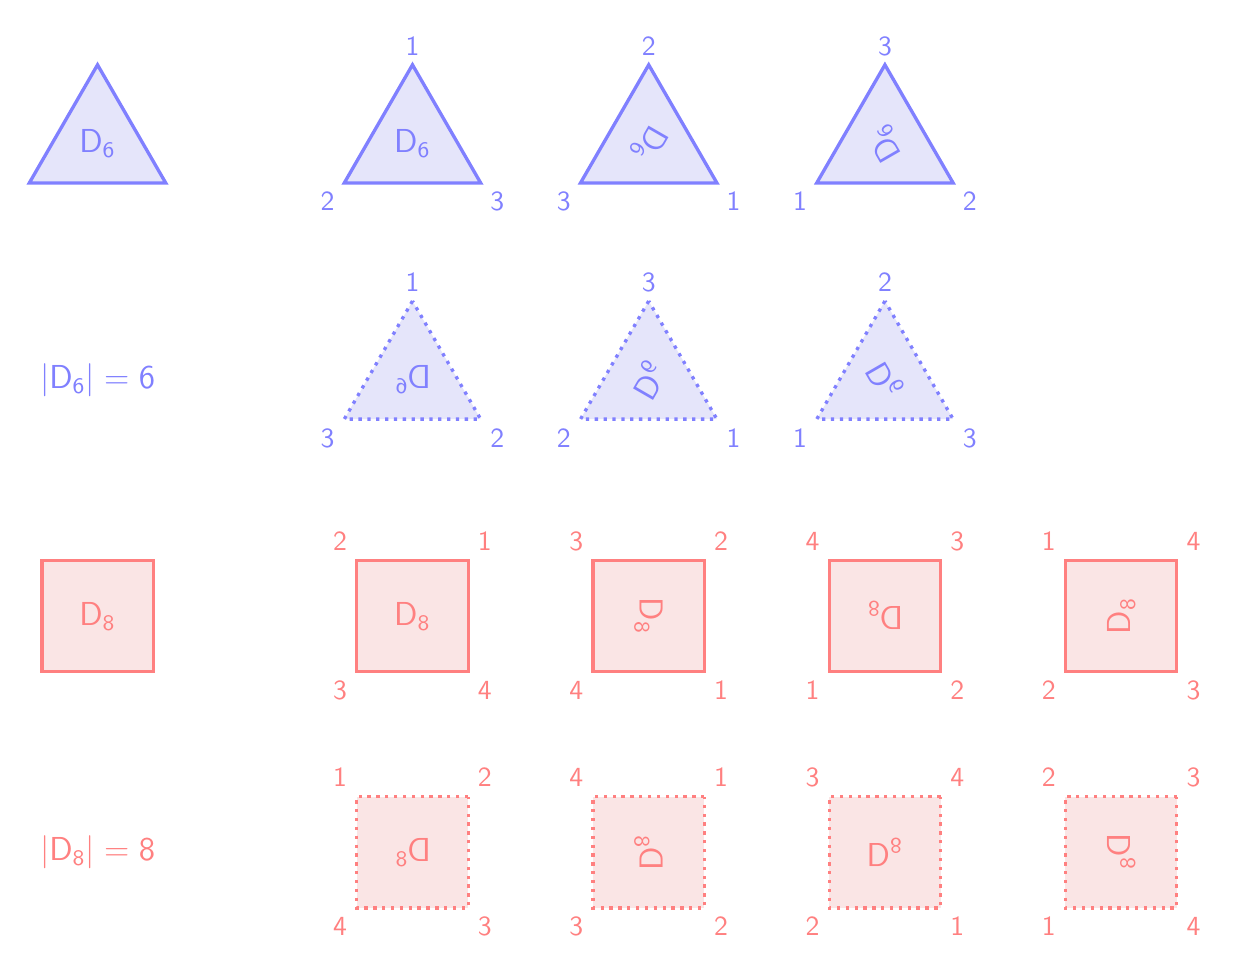
\begin{tikzpicture}
    \coordinate (O) at (0,0);
    \coordinate (A) at (90:1);
    \coordinate (B) at (210:1);
    \coordinate (C) at (330:1);

    \filldraw [draw=blue!50, very thick, fill=blue!80!black!10!] (A) -- (B) -- (C) -- cycle;
    \node at (O) [blue!50] {\large $\mathsf{D_{6}}$};

    \coordinate (O1) at ($(O) + (4,0)$);
    \coordinate (A1) at ($(A) + (4,0)$);
    \coordinate (B1) at ($(B) + (4,0)$);
    \coordinate (C1) at ($(C) + (4,0)$);
    \filldraw [draw=blue!50, very thick, fill=blue!80!black!10!] (A1) -- (B1) -- (C1) -- cycle;
    \node at (O1) [blue!50,rotate=0] {\large $\mathsf{D_{6}}$};
    \node at (A1) [above, blue!50] {$\mathsf{1}$};
    \node at (B1) [below left, blue!50] {$\mathsf{2}$};
    \node at (C1) [below right, blue!50] {$\mathsf{3}$};

    \coordinate (O2) at ($(O1) + (3,0)$);
    \coordinate (A2) at ($(A1) + (3,0)$);
    \coordinate (B2) at ($(B1) + (3,0)$);
    \coordinate (C2) at ($(C1) + (3,0)$);
    \filldraw [draw=blue!50, very thick, fill=blue!80!black!10!] (A2) -- (B2) -- (C2) -- cycle;
    \node at (O2) [blue!50,rotate=-120] {{\large $\mathsf{D_{6}}$}};
    \node at (A2) [above, blue!50] {$\mathsf{2}$};
    \node at (B2) [below left, blue!50] {$\mathsf{3}$};
    \node at (C2) [below right, blue!50] {$\mathsf{1}$};

    \coordinate (O3) at ($(O2) + (3,0)$);
    \coordinate (A3) at ($(A2) + (3,0)$);
    \coordinate (B3) at ($(B2) + (3,0)$);
    \coordinate (C3) at ($(C2) + (3,0)$);
    \filldraw [draw=blue!50, very thick, fill=blue!80!black!10!] (A3) -- (B3) -- (C3) -- cycle;
    \node at (O3) [blue!50,rotate=120] {\large $\mathsf{D_{6}}$};
    \node at (A3) [above, blue!50] {$\mathsf{3}$};
    \node at (B3) [below left, blue!50] {$\mathsf{1}$};
    \node at (C3) [below right, blue!50] {$\mathsf{2}$};

    \coordinate (O4) at ($(O1) + (0,-3)$);
    \coordinate (A4) at ($(A1) + (0,-3)$);
    \coordinate (B4) at ($(B1) + (0,-3)$);
    \coordinate (C4) at ($(C1) + (0,-3)$);
    \filldraw [draw=blue!50, very thick, dotted, fill=blue!80!black!10!] (A4) -- (B4) -- (C4) -- cycle;
    \node at (O4) [blue!50,rotate=0] {\reflectbox{\large $\mathsf{D_{6}}$}};
    \node at (A4) [above, blue!50] {$\mathsf{1}$};
    \node at (B4) [below left, blue!50] {$\mathsf{3}$};
    \node at (C4) [below right, blue!50] {$\mathsf{2}$};

    \coordinate (O5) at ($(O2) + (0,-3)$);
    \coordinate (A5) at ($(A2) + (0,-3)$);
    \coordinate (B5) at ($(B2) + (0,-3)$);
    \coordinate (C5) at ($(C2) + (0,-3)$);
    \filldraw [draw=blue!50, very thick, dotted, fill=blue!80!black!10!] (A5) -- (B5) -- (C5) -- cycle;
    \node at (O5) [blue!50,rotate=-120] {\reflectbox{\large $\mathsf{D_{6}}$}};
    \node at (A5) [above, blue!50] {$\mathsf{3}$};
    \node at (B5) [below left, blue!50] {$\mathsf{2}$};
    \node at (C5) [below right, blue!50] {$\mathsf{1}$};

    \coordinate (O6) at ($(O3) + (0,-3)$);
    \coordinate (A6) at ($(A3) + (0,-3)$);
    \coordinate (B6) at ($(B3) + (0,-3)$);
    \coordinate (C6) at ($(C3) + (0,-3)$);
    \filldraw [draw=blue!50, very thick, dotted, fill=blue!80!black!10!] (A6) -- (B6) -- (C6) -- cycle;
    \node at (O6) [blue!50,rotate=120] {\reflectbox{\large $\mathsf{D_{6}}$}};
    \node at (A6) [above, blue!50] {$\mathsf{2}$};
    \node at (B6) [below left, blue!50] {$\mathsf{1}$};
    \node at (C6) [below right, blue!50] {$\mathsf{3}$};

    \coordinate (O7) at ($(O) + (0,-3)$);
    \node at (O7) [blue!50] {\large $\mathsf{\abs{D_{6}}=6}$};

    % ------------------------------------------------------------
    \coordinate (P) at (0,-6);
    \coordinate (D) at ($(45:1) + (0,-6)$);
    \coordinate (E) at ($(135:1) + (0,-6)$);
    \coordinate (F) at ($(225:1) + (0,-6)$);
    \coordinate (G) at ($(315:1) + (0,-6)$);
    \filldraw [draw=red!50, very thick, fill=red!80!black!10!] (D) -- (E) -- (F) -- (G) -- cycle;
    \node at (P) [red!50] {\large $\mathsf{D_{8}}$};

    \coordinate (P1) at ($(P) + (4,0)$);
    \coordinate (D1) at ($(D) + (4,0)$);
    \coordinate (E1) at ($(E) + (4,0)$);
    \coordinate (F1) at ($(F) + (4,0)$);
    \coordinate (G1) at ($(G) + (4,0)$);
    \filldraw [draw=red!50, very thick, fill=red!80!black!10!] (D1) -- (E1) -- (F1) -- (G1) -- cycle;
    \node at (P1) [red!50,rotate=0] {\large $\mathsf{D_{8}}$};
    \node at (D1) [above right, red!50] {$\mathsf{1}$};
    \node at (E1) [above left, red!50] {$\mathsf{2}$};
    \node at (F1) [below left, red!50] {$\mathsf{3}$};
    \node at (G1) [below right, red!50] {$\mathsf{4}$};


    \coordinate (P2) at ($(P1) + (3,0)$);
    \coordinate (D2) at ($(D1) + (3,0)$);
    \coordinate (E2) at ($(E1) + (3,0)$);
    \coordinate (F2) at ($(F1) + (3,0)$);
    \coordinate (G2) at ($(G1) + (3,0)$);
    \filldraw [draw=red!50, very thick, fill=red!80!black!10!] (D2) -- (E2) -- (F2) -- (G2) -- cycle;
    \node at (P2) [red!50,rotate=-90] {\large $\mathsf{D_{8}}$};
    \node at (D2) [above right, red!50] {$\mathsf{2}$};
    \node at (E2) [above left, red!50] {$\mathsf{3}$};
    \node at (F2) [below left, red!50] {$\mathsf{4}$};
    \node at (G2) [below right, red!50] {$\mathsf{1}$};

    \coordinate (P3) at ($(P2) + (3,0)$);
    \coordinate (D3) at ($(D2) + (3,0)$);
    \coordinate (E3) at ($(E2) + (3,0)$);
    \coordinate (F3) at ($(F2) + (3,0)$);
    \coordinate (G3) at ($(G2) + (3,0)$);
    \filldraw [draw=red!50, very thick, fill=red!80!black!10!] (D3) -- (E3) -- (F3) -- (G3) -- cycle;
    \node at (P3) [red!50,rotate=-180] {\large $\mathsf{D_{8}}$};
    \node at (D3) [above right, red!50] {$\mathsf{3}$};
    \node at (E3) [above left, red!50] {$\mathsf{4}$};
    \node at (F3) [below left, red!50] {$\mathsf{1}$};
    \node at (G3) [below right, red!50] {$\mathsf{2}$};

    \coordinate (P4) at ($(P3) + (3,0)$);
    \coordinate (D4) at ($(D3) + (3,0)$);
    \coordinate (E4) at ($(E3) + (3,0)$);
    \coordinate (F4) at ($(F3) + (3,0)$);
    \coordinate (G4) at ($(G3) + (3,0)$);
    \filldraw [draw=red!50, very thick, fill=red!80!black!10!] (D4) -- (E4) -- (F4) -- (G4) -- cycle;
    \node at (P4) [red!50,rotate=90] {\large $\mathsf{D_{8}}$};
    \node at (D4) [above right, red!50] {$\mathsf{4}$};
    \node at (E4) [above left, red!50] {$\mathsf{1}$};
    \node at (F4) [below left, red!50] {$\mathsf{2}$};
    \node at (G4) [below right, red!50] {$\mathsf{3}$};

    \coordinate (P5) at ($(P1) + (0,-3)$);
    \coordinate (D5) at ($(D1) + (0,-3)$);
    \coordinate (E5) at ($(E1) + (0,-3)$);
    \coordinate (F5) at ($(F1) + (0,-3)$);
    \coordinate (G5) at ($(G1) + (0,-3)$);
    \filldraw [draw=red!50, very thick, dotted, fill=red!80!black!10!] (D5) -- (E5) -- (F5) -- (G5) -- cycle;
    \node at (P5) [red!50,rotate=0] {\reflectbox{\large $\mathsf{D_{8}}$}};
    \node at (D5) [above right, red!50] {$\mathsf{2}$};
    \node at (E5) [above left, red!50] {$\mathsf{1}$};
    \node at (F5) [below left, red!50] {$\mathsf{4}$};
    \node at (G5) [below right, red!50] {$\mathsf{3}$};

    \coordinate (P6) at ($(P2) + (0,-3)$);
    \coordinate (D6) at ($(D2) + (0,-3)$);
    \coordinate (E6) at ($(E2) + (0,-3)$);
    \coordinate (F6) at ($(F2) + (0,-3)$);
    \coordinate (G6) at ($(G2) + (0,-3)$);
    \filldraw [draw=red!50, very thick, dotted, fill=red!80!black!10!] (D6) -- (E6) -- (F6) -- (G6) -- cycle;
    \node at (P6) [red!50,rotate=-90] {\reflectbox{\large $\mathsf{D_{8}}$}};
    \node at (D6) [above right, red!50] {$\mathsf{1}$};
    \node at (E6) [above left, red!50] {$\mathsf{4}$};
    \node at (F6) [below left, red!50] {$\mathsf{3}$};
    \node at (G6) [below right, red!50] {$\mathsf{2}$};

    \coordinate (P7) at ($(P3) + (0,-3)$);
    \coordinate (D7) at ($(D3) + (0,-3)$);
    \coordinate (E7) at ($(E3) + (0,-3)$);
    \coordinate (F7) at ($(F3) + (0,-3)$);
    \coordinate (G7) at ($(G3) + (0,-3)$);
    \filldraw [draw=red!50, very thick, dotted, fill=red!80!black!10!] (D7) -- (E7) -- (F7) -- (G7) -- cycle;
    \node at (P7) [red!50,rotate=-180] {\reflectbox{\large $\mathsf{D_{8}}$}};
    \node at (D7) [above right, red!50] {$\mathsf{4}$};
    \node at (E7) [above left, red!50] {$\mathsf{3}$};
    \node at (F7) [below left, red!50] {$\mathsf{2}$};
    \node at (G7) [below right, red!50] {$\mathsf{1}$};

    \coordinate (P8) at ($(P4) + (0,-3)$);
    \coordinate (D8) at ($(D4) + (0,-3)$);
    \coordinate (E8) at ($(E4) + (0,-3)$);
    \coordinate (F8) at ($(F4) + (0,-3)$);
    \coordinate (G8) at ($(G4) + (0,-3)$);
    \filldraw [draw=red!50, very thick, dotted, fill=red!80!black!10!] (D8) -- (E8) -- (F8) -- (G8) -- cycle;
    \node at (P8) [red!50,rotate=90] {\reflectbox{\large $\mathsf{D_{8}}$}};
    \node at (D8) [above right, red!50] {$\mathsf{3}$};
    \node at (E8) [above left, red!50] {$\mathsf{2}$};
    \node at (F8) [below left, red!50] {$\mathsf{1}$};
    \node at (G8) [below right, red!50] {$\mathsf{4}$};

    \coordinate (P9) at ($(P) + (0,-3)$);
    \node at (P9) [red!50] {\large $\mathsf{\abs{D_{8}}=8}$};
\end{tikzpicture}
\end{center}
\newpage
\thispagestyle{oddpagestyle}
These symmetries are the $n$ rotations about the center through $2\pi/n$ radian,
$0\le i\le n-1$, and the $n$ reflections through the $n$ lines of symmetry.
Now, we only need to define two generators to describe the group $D_{2n}$.
\begin{enumerate}[leftmargin=20pt, itemsep=0pt, topsep=3pt]
    \item {\bf Rotation} $r$: Rotation clockwise about the origin through $2\pi/n$ radian.
    \item {\bf Reflection} $s$: Reflection about the line of symmetry through vertex $1$ and the origin.
\end{enumerate}






\subsection{Symmetric Groups}








\subsection{Matrix Groups}









\subsection{The Quaternion Group}









\subsection{Homomorphisms and Isomorphisms}









\subsection{Group Actions}









\section{Subgroups}
\addtocontents{toc}{\protect\newpage}
\addtocontents{toc}{\protect\thispagestyle{secondpagestyle}}
% ==============================================================================
\end{document}